\documentclass[12pt,a4paper,]{report}

\usepackage[T1,T8K,T8M]{fontenc}
\usepackage[utf8]{inputenc}
\usepackage[english,georgian]{babel}

\usepackage{graphicx}
\usepackage{hyperref}
\usepackage{mathtools}
\usepackage{gensymb}
\usepackage{wrapfig}

\usepackage{subfig}

\hypersetup{
	pdftitle={dummy},
	pdfauthor={Levan Kankadze},
	bookmarksnumbered=true,     
	bookmarksopen=true,         
	bookmarksopenlevel=1,       
	colorlinks=true,
	linkcolor=blue,            
	pdfstartview=Fit,           
	pdfpagemode=UseOutlines,
	bookmarksnumbered, unicode   %ეს უკეთებს ქართულ სარჩევს
	%pdfpagelayout=TwoPageRight
}

\textwidth=16.5cm
\textheight=25cm
\voffset=-2.5cm
\hoffset=-2cm

 %ტექსტის გვერდების გასწორება
\tolerance=10000
\hyphenpenalty=100

\begin{document}

\begin{titlepage}
   \begin{center}
       \vspace*{1cm}

       \textbf{რადიაციული თერაპია}

       \vspace{0.5cm}
        შესავალი
            
       \vspace{1.5cm}

       \textbf{}

       \vfill
            
%       A thesis presented for the degree of\\
%       Doctor of Philosophy
            
       \vspace{0.8cm}
     
       
\includegraphics[width=0.3\textwidth]{images/kiu_logo}
            
       ქუთაისის საერთაშორისო უნივერსიტეტი\\
       საქართველო\\
       2021
            
   \end{center}
\end{titlepage}

\tableofcontents

\chapter{შესავალი}
ამ მცირე კრებულში, მიმოხილულია რადიაციული თერაპიის ძირითადი პრინციპები. ამ ეტაპზე ის უცხოურიდან თარგმანი (ორიგინალი: Amra Ibrahiovic Particles Therapy). 

\pagebreak

\chapter{რა არის რადაციული თერაპია?}
რადიაციული თერაპია არის სიმსივნის მკურნალობის მეთოდი, თუმცა დღესდღეობით რადიაციული თერაპიით შესაძლებელია სხვა დაავადებების განკურნებაც (გული, ...). რადიაციული თერაპია იყენებს ინტენსიური ნაკადების (დამუხტული ნაწილაკების ანდა ელექტრომაგნიტური გამოსხივების) ენერგიას სიმსივნის უჯრედების გასანადგურებლად. ხშირად რადიაციული თერაპია იყენებს რენტგენის სხივებს, თუმცა პროტონების ან სხვა დამუხტული ნაწილაკების გამოყენებაც შეიძლება.

ტერმინი \textbf{რადიაციული თერაპიას} ხშირად ეძახიან  გარე ნაკადებით დასხივებას. ამ ტიპის დასხივებისას, მაღალი ენერგიის ნაკადები გამომსხივებელი მოწყობილობიდან ეცემა სხეულის რომელიმე წინასწარ ზუსტად განსაზღვრულ წერტილს. არსებობს სხვა ტიპის რადიაციული თერაპიას, მაგალითად \textbf{ბრაქითერაპია}\cite{brachytherapy} ამ დროს გამომსხივებელი არის მოთავსებული სხეულის შიგნით. 

რადიაციული თერაპია აზიანებს უჯრედების გენეტიკურ მასალას, რაც პასუხისმგებელია უჯრედის ზრდასა და გაყოფაზე. ცხადია რადიაციულ თერაპია აზიანებს ორივე ჯანმრთელსა და სიმსივნურ უჯრედებს. რადიაციული თერაპიის მიზანია რაც შეიძლება მცირე რაოდენობის ჯანმრთელი უჯრედი დაზიანდეს დასხივებისას. ჯანმრთელ უჯრედებს ასევე შეუძლიათ რადიაციული დაზიანება აღიდგინონ. ამის გამო რადიაციული თერაპიისას მთლიანი დოზის დაყოფა ხდება რამდენიმე მცირე დოზად. ამგვარად სიმსივნური უჯრედები განადგურდებიან ხოლო ჯანმრთელ უჯრედებს ექნებათ საშუალება რომ აღდგნენ.

სიმსივნის გამოსავლენად იყენებენ სხვადასხვა დიაგნოსტიკურ მეთოდებს. მოვიყვანთ რამდენიმეს \textbf{კტ (კომპიუტერული ტომოგრაფია) (CT Computed Tomography)}, \textbf{პეტ (პოზიტრონების ემისიური ტომოგრაფია) (PET (Positron Emission Tomography))}, \textbf{მრტ (მაგნიტურ რეზონანსული ტომოგრაფია) (MRI (Magnetic Resonance Imaging))}. ზოგჯერ ხდება პაციენტის კვლევა რამდენიმე მეთოდით ერთდროულად. დიაგნოსტიკის შემდეგ ხდება მკურნალობის დაგეგვმა და შემდგომ უკვე დასხივება. რადიაციულ თერაპიას წარმართავს რადიაციული ფიზიკოსი ონკოლოგ ექიმთან ერთად. 

\chapter{რადიაციული ერთეულები და დოზები}
როდესაც გამოსხივება (დამუხტული ნაწილაკების ანდა ფოტონების) გადის ნივთიერებაში ურთიერთქმედებს ნივთიერების ატომებთან. რადიაციული თერაპიისას ასეთი ნივთიერებად პაციენტის სხეული განიხილება. ამ ურთიერთქმედების შედეგად ნაწილაკები ტოვებენ ენერგიას გარემოში. დატოვებული ენერგია ნივთიერებაში რიცხვითად ხასიათდება როგორც მიღებული დოზა. 

არსებობს შემდეგი ტიპი დოზების:
	\begin{description}
      \item[$\bullet$] შთანთქმული დოზა  (Absorbed dose)
      \item[$\bullet$] ექვივალენტური დოზა (Equivalent dose)
      \item[$\bullet$] ეფექტური დოზა (Effective dose)
    \end{description}
    
\textit{შთანთქმული დოზა} განისაზღვრება როგორც მაიონიზერებელი გამოსხივების მიერ დატოვებული ენერგია ნივთიერების ერთეულ მასაზე და გამოისახება როგორც $\frac{\text{ჯ}}{\text{კგ}} (J/kg)$. მისი ერთეულია გრეი (Gy-gray) ან 1$\frac{\text{ჯ}}{\text{კგ}} (J/kg)$.

\textit{ექვივალენტური დოზა} განისაზღვრება როგორც შთანთქმული დოზა გამრავლებული რადიაციულ წონის ფაქტორზე.
	\begin{equation}
		H_T = D \times w_R
	\end{equation}
სადაც $H_T$ არის ექვივალენტური დოზა, ხოლო $D$ არის შთანთქმული დოზა და $w_R$ რადიაციული წონის ფაქტორი. ექვივალენტური დოზა იზომება ზივერტებში (Sievert (SV)). რადგანაც $w_R$ არის უგანზომილებო სიდიდე სივერტის განზომილება იგივეა რაც გრეის, თუმცა შთანთქმული დოზისგან რომ განვასხვავოთ შემოტანილია ახალი ერთეული. ცხრილში \ref{tab:rad_weight_factor} მოყვანილია წონითი ფაქტორები სხვადასხვა ტიპის რადიაციებისთვის. 
    \begin{table}[h]
        \centering
        \begin{tabular}{l | l}
             დასხივების ტიპი & დასხივების "წონა" \\
             \hline
             \hline
             რენტგენი & 1 \\
             $\gamma$-zrake(?) & 1 \\
             ელექტრონები და პოზიტრონები & 1 \\
             ნეიტრონები & დამოკიდებულია ენერგიაზე (Energy dependence) \\
             2 მევ-ის პროტონები & 2 \\
             $\alpha$ ნაწილაკები და მძიმე იონები & 20 \\
        \end{tabular}
        \caption{რადიცული წონები}
        \label{tab:rad_weight_factor}
    \end{table}
    
\textit{ეფექტური დოზა} არის დოზა რომელსაც იღებს მთლიანად სხეული, მის გამოსათვლელად საჭიროა, თითოეულ ორგანოზე მიღებული ექვივალენტური დოზა გავამრავლოთ ორგანოს წონით ფაქტორზე და შევკრიბოთ. წონითი ფაქტორი დამოკიდებულია ორგანოს მგრძნობიარობაზე დასხივების მიმართ. ყველაზე მგრძნობიარე ორგანოებია: თვალი, საშვილოსნო და სათესლე ჯირკვლები.
	\begin{equation}
		E = \sum H_T \times w_T
	\end{equation}
სადაც $E$ არის ეფექტური დოზა,  $H_t$ არის ექვივალენტური დოზა და $w_T$ არის ორგანოს წონითი ფაქტორი. 

\chapter{რადიაციული დაზიანება}
სხვადასხვა ენერგიის და სახის გამოსხივება სხვადასხვანაირად მოქმედებს სხეულში. დაბალი ენერგიის ნაწილაკებს გააჩნიათ უფრო დაბალი განჭოლვის უნარი. ამავდროულად სხვადასხვა სახის გამოსხივება იწვევს სხვადასხვა ურთიერთქმედებასა და  სხვადასხვა სახის დაზიანებას ცოცხალი ორგანიზმის უჯრედებში. გამოსხივება პირდაპირ მოქმედებს დნმ-ზე. დნმ-ი შედგება ორი დაკავშირებული პოლინუკლუედური ჯაჭვისგან და წარმოქმნის სპირალს. რადიაციის შედეგად ზიანდება ეს ჯაჭვები და ამის შედეგად შეიძლება უჯრედი სრულად აღდგეს, ან არასწორად აღდგეს ანდა მოკვდეს. ჯანმრთელი უჯრედების დასხივებისას ყველაზე სასურველია პირველი შემთხვევა, თუმცა ყოველთვის ასე არ ხდება, და მეორე ან მესამე შემთხვევა ვითარდება. მეორე შემთხვევა ყველაზე საშიშია რადგანაც, არასწორად აღდგენილი, მუტირებული უჯრედმა შესაძლოა მოგვიანებით იმსივნე გამოიწვიოს. ამიტომაცაა რომ მძიმე იონების და პროტონებით თერაპია არის უფრო მიმზიდველი, მათი დასხივებისას ზიანდება ორივე ჯაჭვი და იწვევს უჯრედის სრულ სიკვდილს, ამიტომაც უჯრედის მუტაცია აღარ ხდება, განსხვავებით ფოტონებით დასხივებისას, ამ დროს ზიანდება მხოლოდ ერთი ჯაჭვი რაც ტოვებს უჯრედის მუტაციის რისკს. ამავდროულად სიმსივნურ უჯრედებს არ გააჩნიათ აღდგენის უნარი და დნმ-ის დაზიანებისას ისინი კვდებიან, მაგრამ გარკვეულ შემთხვევებში სიმსივნე მედეგია ფოტონური დასხივების მიმართ. ამ მიზეზთა გამო პროტონებსა და ნახშირბადის ბირთვებს აქვთ მეტი ალბათობა სიმსივნური უჯრედების განადგურებისა.

	\begin{figure}[htp]
	    \centering
        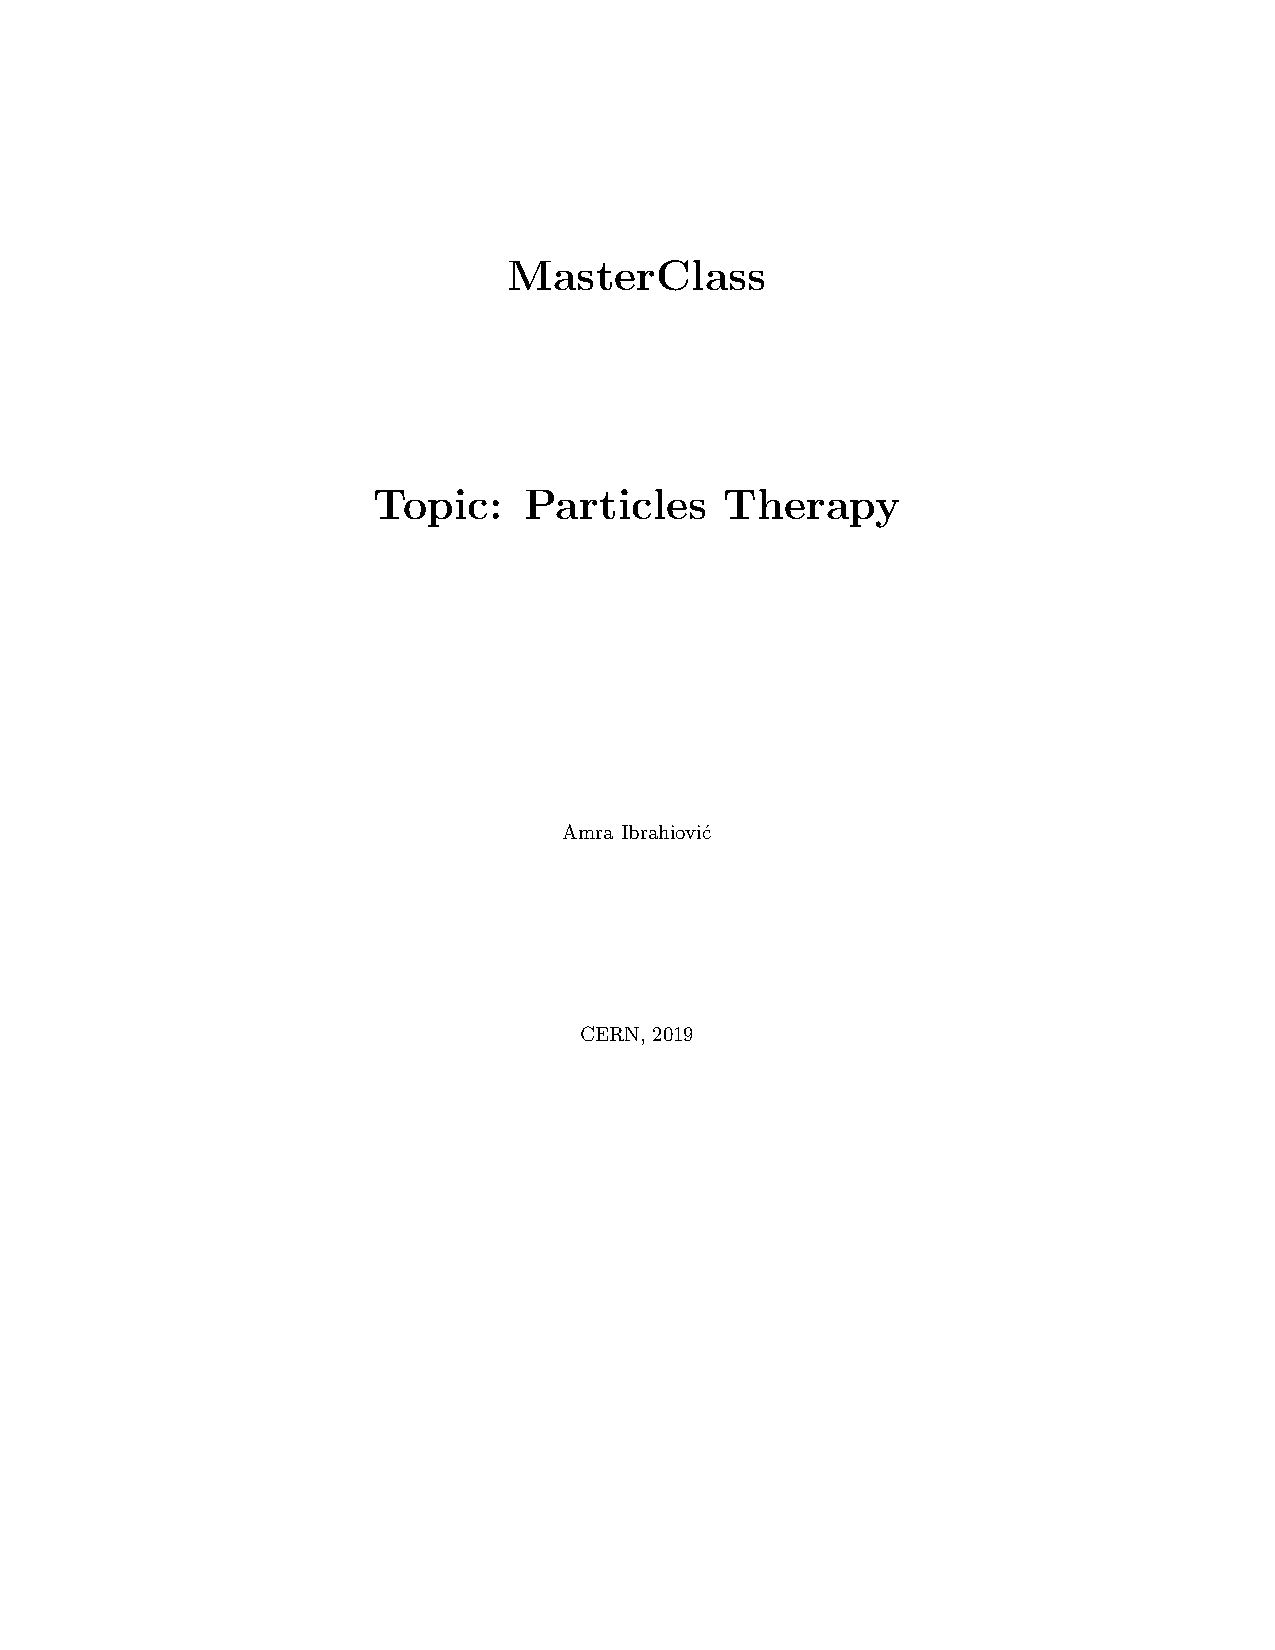
\includegraphics[width = 6cm]{images/Radiotherapy.jpg}
        \caption{ჰიერარქიული ნახატი უჯრედისა, ბირთვისა, ნუკლეუსის და დნმ-ის.}
        \label{fig:1}
    \end{figure}

\section{ფბე (ფარდობითი ბიოლოგიური ეფექტურობა) RBE (relative biological effectiveness)} 
როგორც უკვე ავღნიშნეთ სხვადასხვა ტიპის გამოსხივება სხვადასხვა რაოდენობის გამოსხივებას ტოვებს ბიოლოგიურ ქსოვილებში. ფბე (ფარდობითი ბიოლოგიური ეფექტურება) არის ფარდობითი ზომა რადიაციული დაზიანებისა
რეფერენს რადიაცია ჩვეულებრივ არის 220 
	\begin{figure}[htp]
	    \centering
        \includegraphics[width = 8cm]{images/Picture1.png}
        \caption{caption.}
        \label{fig:1}
    \end{figure}
    
\chapter{რადიაციული თერაპიის დაგეგმვა (Radiation Treatment Planing)}
\section{ფანტომები (Phantoms)}
ძირითადი დოზების განაწილების მონაცემები გაზომილია წყლის ფანტომში (water phantom), რომელიც საკმაოდ ახლოსაა კუნთისა და სხვა რბილი რადიაციული შთანთქმის და გაფანტვის რეალურ მნიშვნელობებთან. კიდევ მიზეზი რის გამოც ირჩევენ წყლის ფანტომს, იგი უნივერსალურია და ადვილად შეიძლება რადიციული თვისებების გამეორება (?) [Another reason for the choice of water as a phantom material is that it is universally available with reproducible radiation properties]. რამდენადაც ყოველთვის არაა შესაძლებელი გამოსხივების დეტექტორების წყალში განთავსება, არსებობს მყარი ფანტომები რომლებსაც შეუძლიათ ჩაანაცვლონ წყალი. იდეალურ შემთხვევაში მოცემულ ნივთიერებას რომ იყოს ქსოვილების ანდა წყლის ექვივალენტი, მას უნდა გააჩნდეს იგივე: ეფექტური ატომური რიცხვი, ელექტრონების რიცხვი თითოეულ გრამ ნივთიერებაზე და მასური სიმკვრივე. თუმცა, რადგან კომპტონის ეფექტი არის ძირითადი ურთიერთქმედება მეგავოლტიანი ფოტონების (photon beams in the clinical range,) ნაკადისთვის. ასე შემთხვევაში რომ იყოს ნივთიერება წყლის ექვივალენტი საჭიროა ქონდეს იგივე ელექტრონული სიმკვრივე (ელექტრონების რაოდენობა კუბურ სანტიმეტრზე).

	\begin{figure}[h]%
    	\centering
    	\subfloat[\centering მყარი ფანტომი]{{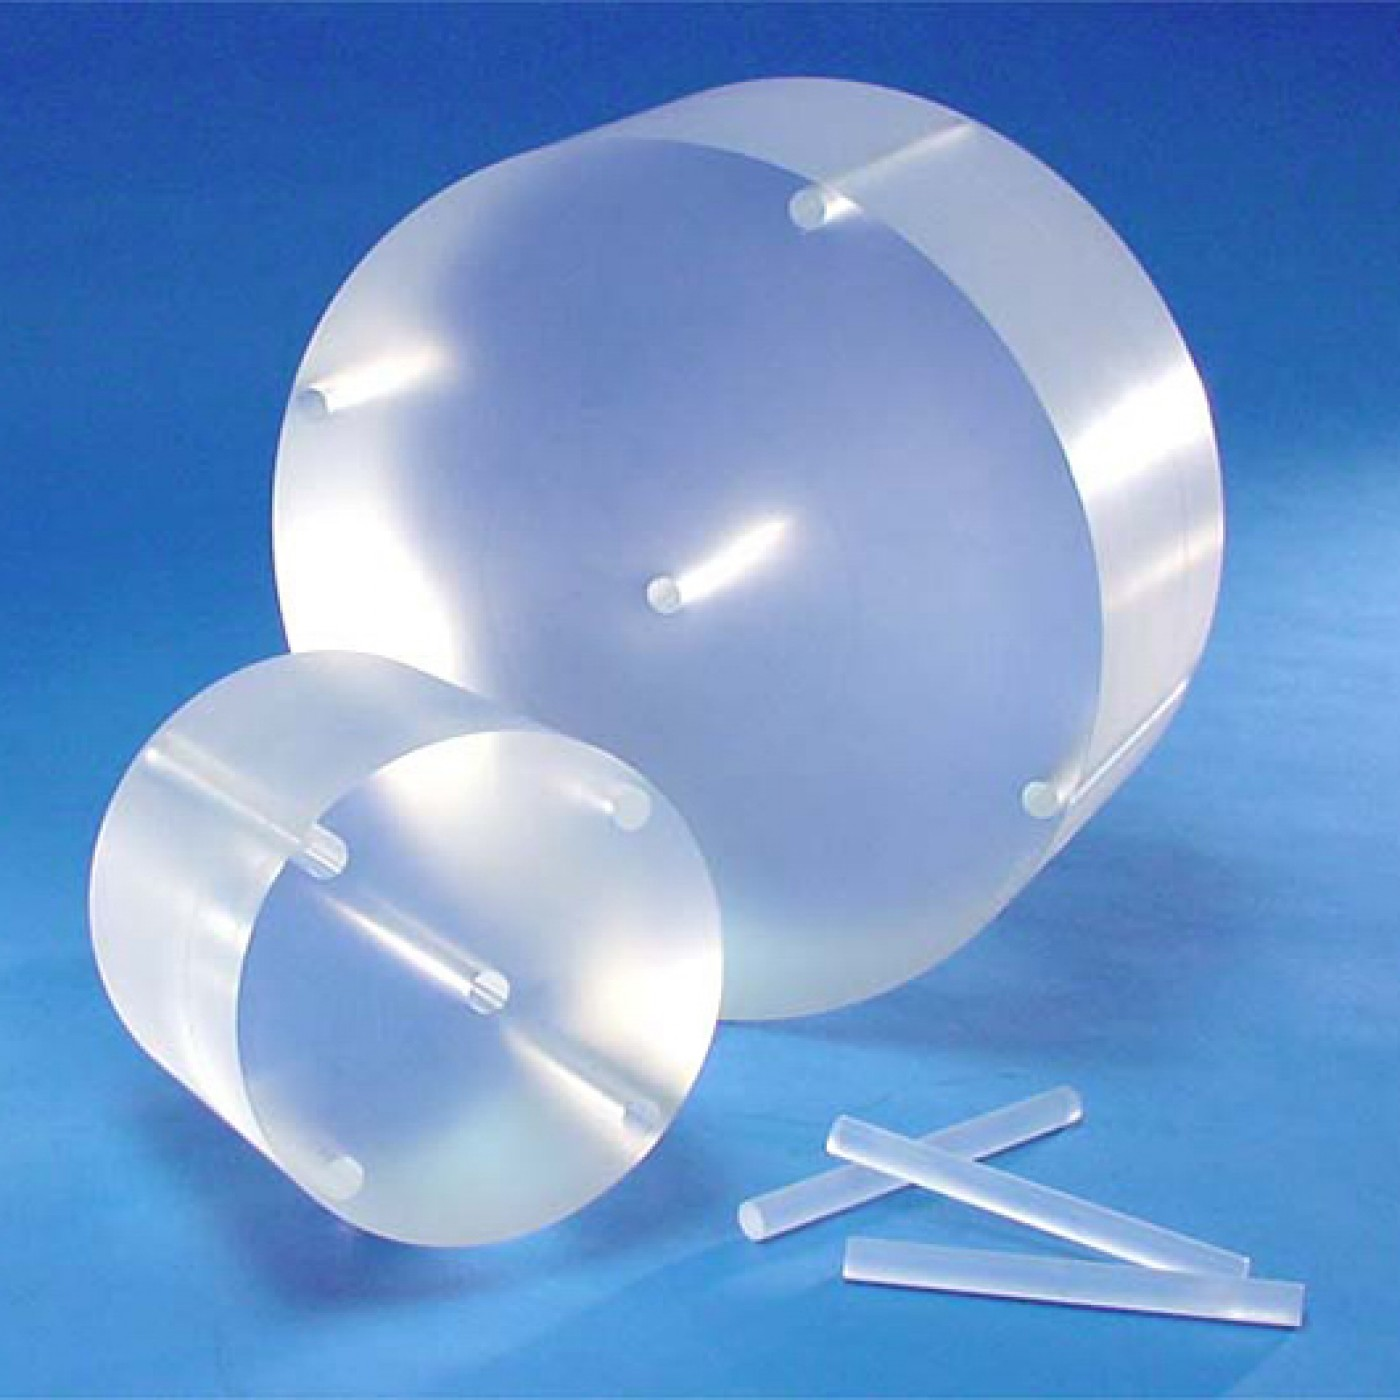
\includegraphics[width=6cm]{images/phantom_a} }}%
    	\qquad
    	\subfloat[\centering წყლის ფანტომი]{{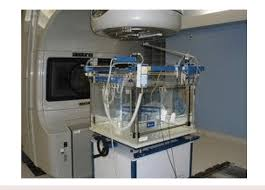
\includegraphics[width=9cm]{images/phantom_b} }}%
    	\caption{ფანტომები}%
    	\label{fig:phantom}%
	\end{figure}

\section{სიღრმისეული დოზის განაწილება (Depth Dose Distribution)}
როგორც კი სხივი მოხვდება პაციენტში ( ან ფანტომში), შთანთქმული დოზის სიდიდე მერყეობს სიღრმის მიხედვით, რაც დამოკიდებულია სხვადასხვა 
მდგომარეობებზე: სხივის ენერგია, სიღრმე, ველის ზომა, წყაროდან დაშორება და სხივის კოლიმაციის სისტემა. ამრიგად, პაციენტში დოზის გაანგარიშება ხდება, ყველა აღნიშნული პარამეტრის გათვალისწინებით, რადგანაც ეს პარამეტრები გავლენას ახდენენ დოზის განაწილებაზე სიღრმის მიხედვით. დოზის დაანგარიშებისათვის, ძირითადი ნაბიჯია წარმოვადგინოთ მისი განაწილება სიღრმეში სხივის გასწვრივ, ცენტრალური აქსიალური ღერძის მიმართ. 
ფანტომებში სხვადასხვა დეტექტორების( იონიზაციის კამერები, ნახევარგამტარი დეტექტორები, თლდ( თერმოლუმინესცენციური დოზიმეტრი)),  საშუალებით ხდება სიღრმისეული დოზის განაწილების გაზომვა. სხვადასხვა სახის სხივს აქვს, განსხვავებული დოზის განაწილება სიღრმეში. იზოდოზების ცხრილში, მოცემულია სხივის შემადგენლობის მიხედვით აგებული მრუდი, რომელიც წარმოადგენს სხივისა და ჩაღწევის სიღრმის დამოკიდებულების 
აქსიალურ ფუნქციას, სიღრმისეული დოზის მნიშვნელობა მრუდებზე დანორმირებულია, აქსიალურ ღერძზე მაქსიმალური დოზის შესაბამისი წერტილის გასწვრივ. ველის ზომა შეიძლება გამოვყოთ, როგორც გეომეტრიულად ასევე დოზიმეტრულად. ველის გეომეტრიული ზომა განისაზღვრება, როგორც „ პროექცია, სიბრტყის მართობული სხივის ღერძისა, კოლიმატორის დისტალური ნაწილის ბოლოდან წყაროს წინა ცენტრალურ ნაწილამდე. ეს განსაზღვრება ჩვეულებრივ შეესაბამება სინათლის ლოკალიზატორის მიერ განსაზღვრულ ველს, რომელიც მოწყობილია ისე, რომ სინათლის წერტილოვანი წყარო მდებარეობს ზუსტად ცენტრში და მისი მდებარეობა შეესაბამება გამომსხივებელი წინა ზედაპირს. 
	\begin{figure}[h]
	    \centering
        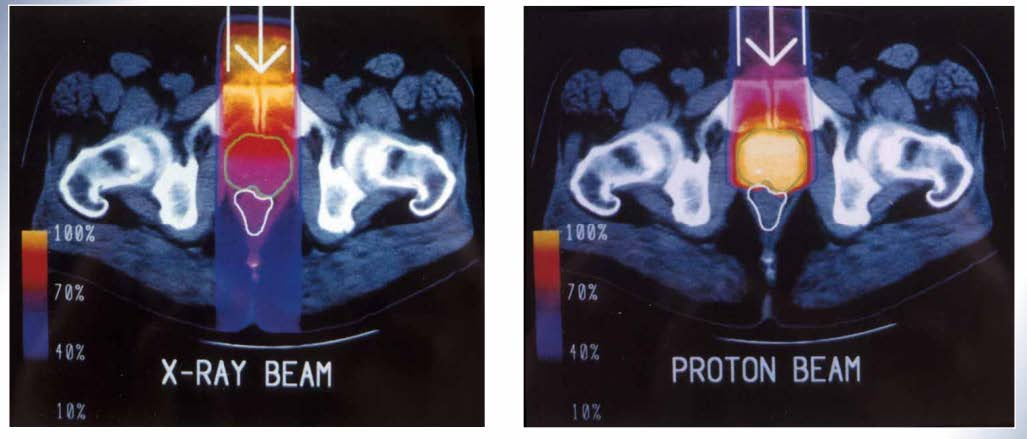
\includegraphics[width = 15cm]{images/depth_dose_distribution_01}
        \caption{caption.}
        %\label{fig:}
    \end{figure}
დოზიმეტრული ან ფიზიკური, ველის ზომა არის მანძილი, რომელსაც კვეთს მოცემული იზოდოზის მრუდი (ჩვეულებრივ, აღებულია $50$ იზოდოზა). 
თუ სხვაგვარად არ არის მითითებული, ტერმინი ველის ზომა აღნიშნავს ველის გეომეტრიულ ზომას. ასევე, ველის ზომა განისაზღვრება წინასწარ განსაზღვრული მანძილით, როგორიცაა SSD(sourse surface distance) წყაროს ზედაპირიდან დაშორების მანძილი, ან წყაროს ღერძამდე მანძილი (SAD-sourse axise distance). ეს უკანასკნელი ტერმინი არის მანძილი წყაროდან განტრის ბრუნვის ღერძამდე, რომელიც ცნობილია როგორც იზოცენტრი.

	\begin{figure}[h]%
    	\centering
    	\subfloat[\centering ...]{{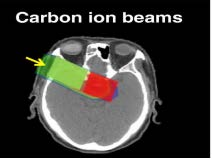
\includegraphics[width=6cm]{images/depth_dose_distribution_02a} }}%
    	\qquad
    	\subfloat[\centering ...]{{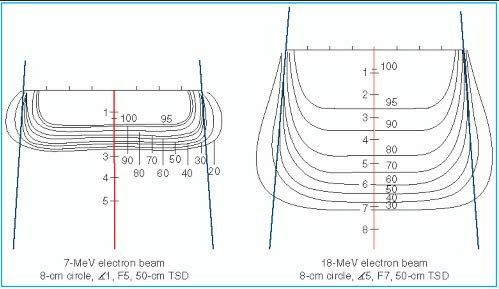
\includegraphics[width=8cm]{images/depth_dose_distribution_02b} }}%
    	\caption{ფანტომები}%
    	\label{fig:phantom}%
	\end{figure}

\section{მრავალჯერადი ველები (Multiple Fields)}
მკურნალობის ერთ-ერთი ყველაზე მნიშვნელოვანი მიზანია მისი დაგეგმვა ისე რომ მაქსიმალური დოზა მივაწოდოთ სიმსივნეს და მინიმალური დოზა გარშემორტყმულ ქსოვილებს, ამ პროცესს ოპტიმიზაცია ეწოდება. გარდა ამისა, დოზის ერთგვაროვნება სიმსივნის მოცულობის შიგნით და რისკ ორგანოების ნაკლები დაზიანებაც გეგმის განხილვისას განსაკუთრებული მსჯელობის საგანია. 
არსებობს რამოდენიმე სტრატეგია ჩვენი მიზნის მისაღწევად:
	\begin{description}
      \item[$\bullet$] შესაბამისი ზომის ველების გამოყენება
      \item[$\bullet$] ველების რაოდენობის გაზრდა
      \item[$\bullet$] სხივის შესაბამისი მიმართულებების შერჩევა
      \item[$\bullet$] სხივის წონის მორგება (დოზის წვლილი ცალკეული ველებიდან)
      \item[$\bullet$] სხივის შესაბამისი ენერგიის გამოყენება
      \item[$\bullet$] სხივის მოდიფიკატორების გამოყენება,როგორებიცაა სოლი ფილტრები და კომპენსატორები
    \end{description}
იმ პარამეტრების მოპოვება,რომელიც იძლევა ოპტიმალურ გეგმას ხელით მუშაობის დროს საკმაოდ შრომატევადია, მაგრამ ახლა უკვე ხელმისაწვდომია მკურნალობის დაგეგმვის კომპიუტერები, რომლებსაც შეუძლიათ სამუშაოს სწრაფად და ზუსტად შესრულება. ამ სისტემებით დამგეგმარებელს შეუძლია მყისიერი მოდიფიკაცია, გამოთვლა და შესწავლა ნებისმიერი გეგმის, რაც საშუალებას აძლევს კლინიკურად საუკეთესო გეგმა აარჩიოს.

	\begin{figure}[!h]
	    \centering
        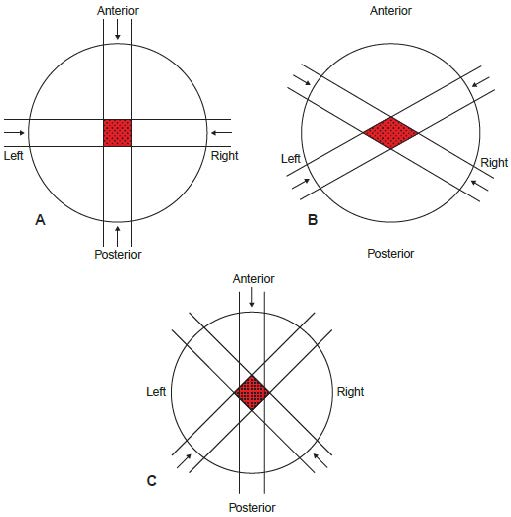
\includegraphics[width = 15cm]{images/multiple_fields_01}
        \caption{caption.}
        %\label{fig:}
    \end{figure}

	\begin{figure}[!h]
	    \centering
        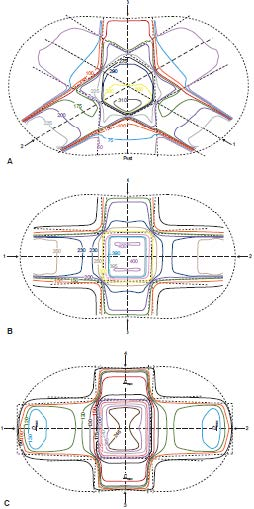
\includegraphics[width = 11cm]{images/multiple_fields_02}
        \caption{Examples of multiple field plans. A: Three field B: Four fi eld C: Four field.}
        %\label{fig:}
    \end{figure}

\section{სტაციონარული სხივები (Stationary Beams)}
დასხივების იზოცენტრული ტექნიკა გულისხმობს აპარატის იზოცენტრის განთავსებას პაციენტის სიღრმეში და სხივების სხვადასხვა მიმართულებით გაბნევას. წყაროდან იზოცენტრამდე მანძილი (ან როგორც ვეძახით SAD (source to axis distance)), სხივის მიმართულების მიუხედავად მუდმივი რჩება.

\section{ბრუნვითი თერაპია (Rotation Therapy)}
ბრუნვითი თერაპია არის იზოცენტრული მეთოდის ერთ-ერთი სახეობა, სადაც სხივი უწყვეტად ბრუნავს პაციენტის თავზე , ან პაციენტს აბრუნებენ ფიქსირებული სხივის გარშემო. ასევე ეს ტექნიკა გამოიყენება : საყლაპავი მილის, შარდის ბუშტის, პროსტატის ჯირყვლის, საშვილოსნოს ყელის და ტვინის სიმსივნეების სამკურნალოდ.  ამ მეთოდს გააჩნია მცირედი უპირატესობა იზოცენტრულ მეთოდზე, როცა გამოყენებულია რამოდენიმე სხივი. მაგალითად: საყლაპავი მილის მკურნალობა კარგად , შესაძლებელია როგორც იზოცენტრული მეთოდით ასევე ფიქსირებული წყაროს გამოყენებით, ასევე სამი ველის გამოყენებით.  პროსტატის ჯირყვლების და შარდის ბუშტის მკურნალობა შესაძლებელია ოთხი ველის(ნაკადი) გამოყენებით.  ზოგჯერ გამოყენებულია პარალელური ურთიერთსაწინააღმდეგო ველები. ხოლო თვინის მკურნალობა შესაძლებელია სამი ან ორი ველის გამოყენებით.

\chapter{ICRU Volumes (International Commission on Radiation Units and Measurements)}
\section{სიმსივნის მთლიანი მოცულობა}

	\begin{wrapfigure}{l}{0.5\textwidth}
	    \centering
        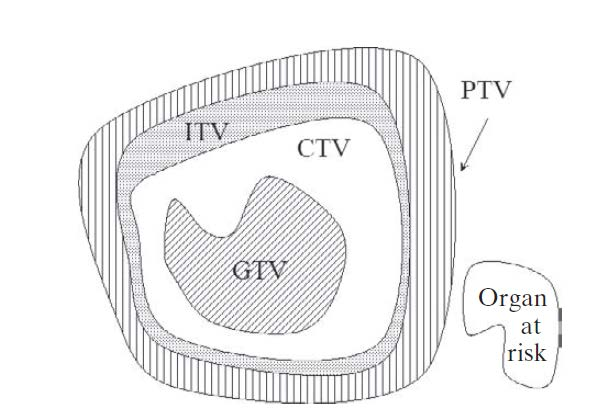
\includegraphics[width=.7\linewidth]{images/gross_tumor_volume}
        \caption{caption.}
        %\label{fig:}
    \end{wrapfigure}

სიმსივნის მთლიანი მოცულობა არის ის საჩვენებელი მოცულობა ,რომელსაც მოიცავს მთლიანი სიმსივნე. ეს შედგება თვითონ სიმსივნური წარმონაქმნისგანს, მეტასტაზური ლიმფადენოპათიისგან,  და სხვა მეტასტაზებისგან. სიმსივნის მთლიანი მოცულობის გამიჯვნა შესაძლებელია თუ სიმსივნე თვალით ჩანს, იგრძნობა ხელით შეხებისას ან ჩანს დასკანერების შედეგად. სიმსივნის მთლიან მოცულობას ვერ განვსაზღვრავთ თუ მისი დიდი ნაწილი არის ამოკვეთილი ან სიმსივნის გარსი არის წინასაოპერაციო. 

\section{კლინიკური სამიზნე მოცულობა (Clinical Target Volume)}
კლინიკური სამიზნე მოცულობა (CTV) შედგება დემონსტრირებული სიმსივნისგან, თუ ახლავს (აქვს)  ნებისმიერი სხვა ქსოვილი მასზე სავარაუდოდ არსებული სიმსივნით.  ამიტომ ზემოთხსენებული წარმოადგენს სიმსივნის რეალურ ზომასა და მდებარეობას. CTV-ის დახაზვა გვაძლევს მეტ ვარაუდს,  რომ იქ არ არის სიმსივნური უჯრედები ამ მოცულობის  მიღმა. CTV-მ უნდა მიიღოს ადეკვატური დოზა თერაპიული მიზნის მისაღწევად.

\section{შიდა სამიზნე მოცულობა (Internal Target Volume)}
ICRU ანგარიში 62 (15) რეკომენდაციას იძლევა, რომ დაემატოს შიდა ზღვარი (IM). CTV შიდა ფიზიოლოგიური მოძრაობების და ზომის ცვალებადობის კომპენსაციისთვის  გამოიყენება, CTV-ის ფორმა და პოზიცია თერაპიის დროს შიდა ეტალონთან მიმართებაში  აისახება წერტილით და მისი შესაბამისი კოორდინატთა სისტემით. მოცულობა, რომელიც  მოიცავს CTV-ის ამავე მინდვრებით ეწოდება შიდა სამიზნე მოცულობა (ITV).

\section{დაგეგმვის სამიზნე მოცულობა (Planning Target Volume)}
მოცულობა, რომელიც მოიცავს CTV IM-ს    , ასევე დაყენების ზღვარს (SM). პაციენტის მოძრაობა და დაყენების გაურკვევლობა ეწოდება დაგეგმვის  სამიზნე მოცულობას (PTV) . PTV-ის დასახაზად, IM და SM არ არის დამატებული  ხაზობრივად,  მაგრამ არის კომბინირებული საკმაოდ დიდი მიახლოებით.  ზღვარი CTV-ის გარშემო ნებისმიერი მიმართულებით , საკმარისად დიდი იყოს შიდა მოძრაობების კომპენსირებისთვის და პაციენტის მოძრაობისთვის და დაყენების გაურკვევლობებისათვის.

\section{დაგეგმვა რისკის ქვეშ მყოფი ორგანული მოცულობის (Planning Organ at Risk Volume)}
რისკის ქვეშ მყოფი ორგანო(ები) საჭიროებს ადეკვატურ დაცვას, ისევე როგორც CTV საჭიროებს  ადეკვატურ მკურნალობას. მას შემდეგ რაც OR-ი იდენტიფიცირებული იქნება, მინდვრები უნდა დაემატოს და მისი მოძრაობები დაკონპენსირდება, როგორც შიდა, ასევე დაყენების საზღვრებზე. ამრიგად, ანალოგიურად PTV დაყენება, საჭიროა გამოიკვეთოს რისკის ქვეშ მყოფი საგეგმო ორგანოს (PRV) დასაცავად ან ეფექტურობისათვის. ნახაზი სქემატურად ასახავს PTV-ს გამოკვეთის პროცესს და PRV. ეს პროცესი მიზნად ისახავს რადიაციული ონკოლოგის მეთოდურად და ანალიტიკურად დაფიქრებას სამიზნეების და რისკის ქვეშ მყოფი ორგანოების დასახვისას. თუმცა აბსოლუტური სიზუსტის გარანტია არც ერთ შემთხვევაში არ გევქნება, ამ მიდგომის მიზანია შეცდომების მინიმუმამდე შემცირება დეტალებზე ყურადღების გამახვილებით. ასევე მნიშვნელოვანია აღვნიშნოთ, რომ პრაქტიკოსებს შორის საერთოა ხაზვის ტენდენცია.
GTV-ზე დაფუძნებული სამიზნე მოცულობები არსებობს მცირე ზღვრებით სუბკლინიკური დაავადების ორგანოების მოძრაობის ან დაყენების გაურკვევლობის გათვალისწინებით.კონფორმული გამოსხივება ე.წ. თერაპია “ორპირიანი იარაღია“ რითიც გეგმის შესაბამისობის მაღალი ხარისხი შეიძლება შეიქმნას გეოგრაფიული გამოტოვების დიდი ალბათობით.  ამიტომ დიდი სიფრთხილეა საჭირო PTV და PRV დიზაინში მუშაობისას. ასევე მნიშვნელოვანია ვიცოდეთ შეზღუდვების სისტემა, რასაც წარმოადგენს და ვიცოდეთ მისი შესაძლებლობები.

\section{დამუშავებული მოცულობა (Treated Volume)}
დამატებითი მინდვრები უნდა იყოს გათვალისწინებული სამიზნე მოცულობის გარშემო, მკურნალობის ტექნიკის შეზღუდვებით. ამრიგად, მინიმალური სამიზნე დოზა უნდა იყოს წარმოდგენილი იზოდოზური ზედაპირით, რომელიც ადეკვატურად ფარავს PTV-ს საზღვრებს. ამ იზოდოზური ზედაპირით შემოსაზღვრულ მოცულობას დამუშავებული მოცულობა ეწოდება. დამუშავებული მოცულობა, ზოგადად, უფრო დიდია ვიდრე დაგეგმვის სამიზნე მოცულობა და დამოკიდებულია მკურნალობის კონკრეტულ ტექნიკაზე.

\section{დასხივებული მოცულობა (Irradiated Volume)}
ქსოვილის მოცულობა, რომელიც იღებს მნიშვნელოვან დოზას (მაგ., მითითებული სამიზნის $50\%$ დოზა) ეწოდება დასხივებულ მოცულობას. დასხივებული მოცულობა უფრო დიდია ვიდრე დამუშავებული მოცულობა და დამოკიდებულია გამოყენებული მკურნალობის ტექნიკაზე.

\section{მაქსიმალური სამიზნე დოზა (Maximum Target Dose)}
უმაღლეს დოზას სამიზნე არეში ეწოდება მაქსიმალური სამიზნე დოზა, გათვალისწინებული ეს დოზა მოიცავს მინიმალურ ფართობს 2 sm2. უფრო მაღალი დოზით 2 სმ2-ზე ნაკლები ფართობები შეიძლება იგნორირებული იყოს მაქსიმალური სამიზნე დოზის მნიშვნელობის განსაზღვრისას.

\section{მინიმალური სამიზნე დოზა (Minimum Target Dose)}
მინიმალური სამიზნე დოზა არის ყველაზე დაბალი აბსორბირებული დოზა სამიზნე ზონაში. 

\section{საშუალო სამიზნე დოზა (Mean Target Dose)}
თუ დოზა გამოითვლება სამიზნე ზონაში თანაბრად განაწილებულ დისკრეტულ წერტილების დიდ რაოდენობაზე, საშუალო სამიზნე დოზა არის შთანთქმის საშუალო დოზის მნიშვნელობები ამ წერტილებში. 

\section{ცხელი წერტილები (Hot Spots)}
ცხელი წერტილი არის ფართობი რომელიც არის მიზნის გარეთ და იღებს უფრო მეტ დოზას ვიდრე მიზნისთვისაა განსაზღვრული. როგორც მაქსიმალური სამიზნე დოზა, ცხელი წერტილი იძენს სამედიცინო აზრს თუ ის ფარავს სულ მცირე 2~$\text{სმ}^2$ ფართობს.

\chapter{მონაცემთა მოგროვება (Data Acquisition)}
სხეულის კონტურებისა და შინაგანი სტრუქტურების შეგროვება საუკეთესოდ სრულდება 3D მოცულობითი გამოსახულებით (კომპიუტერული ტომოგრაფია CT, მაგნიტო რეზონანსული გამოსახულება (MRI) და სხვა..). სკანირება ტარდება მკურნალობის დაგეგმვის მიზნით, ამ დროს პაციენტი მოთავსებულია ზუსტად ისე როგორც მკურნალობის დროს უნდა იყოს. 3D მკურნალობის დაგეგმვისას მონაცემები მოპოვებულია სურათებით და მიღებულია როგორც მკურნალობა-დაგეგმვის ნაწილი. თუმცა, იმ შემთხვევებისთვის, როდესაც 3-D მკურნალობის დაგეგმვა საჭიროდ არ ითვლება ან სხეულის კონტურების მიღება ხელითაც შეგვიძლია, კონტურინგისთვის გამოიყენება მექანიკური ან ელექტრომექანიკური მეთოდები.


\section{მაგნიტურ-რეზონანსული ტომოგრაფია (Magnetic Resonance Imaging)}
MRI ჩამოყალიბდა კომპიუტერული ტომოგრაფიის პარალელურად, ვიზუალიზაციის მძლავრ მოდალად. ოსწონს CT, ის უზრუნველყოფს ანატომიურ სურათებს მრავალ სიბრტყეში. ვინაიდან CT უზრუნველყოფს ძირითადად განივი ღერძული გამოსახულებები (რომლების შემდგომი დამუშავება შესაძლებელია რეკონსტრუქციისთვის სურათები სხვა სიბრტყეში ან სამ განზომილებაში), MRI შეიძლება გამოყენებულ იქნას უშუალოდ სკანირებისთვის ღერძულ, საგიტალურ, კორონალურ ან ირიბ სიბრტყეებში. ეს შესაძლებელს ხდის მოპოვებას ოპტიმალური ხედები დიაგნოსტიკური ინტერპრეტაციის გასაუმჯობესებლად ან მიზნობრივი განსაზღვრისთვ ს რადიოთერაპია. სხვა უპირატესობები CT-სთან შედარებით მოიცავს მაიონებელი საშუალებების გამოყენებას რადიაცია, მაღალი კონტრასტი და რბილი ქსოვილების სიმსივნეების უკეთესი გამოსახულება. ზოგიერთი უარყოფითი მხარეები CT-თან შედარებით მოიცავს დაბალ სივრცულ გარჩევადობას.



\section{პოზიტრონ ემისიური ტომოგრაფია (Positron emission tomography)}
პოზიტრონ ემისიური ტომოგრაფია (PET) იძლევა ფუნქციურ სურათებს, რომლებსაც შეუძლიათ განასხვავონ ავთვისებიანი სიმსივნეები და მიმდებარე ჯანსაღი ქსოვილები ერთმანეთისგან. ეს მონაცემები შეიძლება გაერთიანდეს იმ ანატომიურ ინფორმაციასთან რომელსაც კომპიუტერული ტომოგრაფია(CT) მოგვცემს და ისინი შეავსებენ ერთმანეთს. ორივე მოდელირების ერთ სისტემად გაერთიანებამ საფუძველი ჩაუყარა PET/CT ს ჩამოყალიბებას.

\chapter{პაციენტის პოზიციისა და იმობილიზაციის ხელსაწყოები მკურნალობისას (Patient treatment position and immobilization devices)}
პაციენტის მკურნალობის პოზიციაზე და განთავსებაზეა დამოკიდებულია დასხივების სიზუსტე.შესაძლებელია ზოგიერთ შემთხვევაში მკურნალობის დროს საჭირო იყოს სპეციალური მოწყობილობები სწორი პოზიციის შესანარჩუნებლად, ან არის შემთხვევები, როცა დასხივების დროს არ საჭიროებს პაციენტი სპეციალურ მოწყობილობებს იმმობილიზაციისთვის
ძირითადად იმობილიზაციის ხელსაწყოებს აქვთ ორი დანიშნულება:
	\begin{description}
      \item[$\bullet$] მკურნალობის დროს პაციენტის იმობილიზაცია
      \item[$\bullet$] უზრუნველყოს პაციენტის პოზიციის საიმედო საშუალება და სიმულაცია მკურნალობამდე ან ერთი მკურნალობიდან მეორემდე.
    \end{description}
სიმულაცია მკურნალობამდე ან ერთი მკურნალობიდან მეორემდე.
უმარტივესი იმობილიზაციის საშუალებებია ნიღბის ლენტი, ველკროს ქამრები და ელასტიკური სახვევები.  საწყისი იმობილიზაციის საშუალებები რადიოთერაპიაში გამოიყენება თავის მოსათავსებლად, რომელიც ისეა ფორმირებული, რომ მჭიდროდ მოერგოს პაცინტს თავსა და კისრის არეში, რაც საშუალებას აძლევს პაციენტმა თავი იგრძნოს კომფორტულად სამკურნალო მაგიდაზე. თანამედროვე რადიოგრაფია მოითხოვს დამატებით იმობილიზაციის საშუალებებს მკურნალობის პროცესში. როდესაც პაციენტს მკურნალობა უტარდება თავის არეში უმეტესად გამოყენებულია პლასტიკური ნიღბები, რომლებიც იმეორებს პაციენტის თავის მოყვანილობას და უზრუნველყოფს მის ფიქსაციას.
ნიღბები და პლასტიკური თეფშები გამოიყენება თვითონ მაგიდაზე დასამაგრებლად, რათა მოხდეს პაციენტის უმოძრაო მდგომარეობაში გაჩერება პლევრისა და გულმკერდის არის მკურნალობის პროცესის დროს.
ვაკუუმზე დაფუძნებული საშუალებები პოპულარულია მათი მრავალჯერადი გამოყენების გამო. ძირითადად, პაწაწინა პოლისტიროლის ბურთულებით სავსე ბალიში მოთავსებულია სამკურნალო უბნის გარშემო და ვაკუუმ ტუმბოს საშუალებით ბალიშზე ტოვებს პაციენტის ფორმას ანაბეჭდად. შედეგი არის ის, რომ პაციენტი შეიძლება იყოს მჭიდროდ და ზუსტად მოთავსებული ბალიშზე ყოველი მკურნალობის წინ.
სხვა სისტემა, მსგავსი კონცეფციით, იყენებს ქიმიური რეაქცია ბალიშში არსებულ რეაგენტებს შორის, რათა შეიქმნას პაციენტის ზუსტი ფორმა. სპეციალური ტექნიკა, როგორიცაა სტერეოტაქსიური რადიოქირურგია, მოითხოვს ისეთი მაღალი დონის სიზუსტეს, რომ ჩვეულებრივი იმობილიზაციის ტექნიკა შეუსაბამოა.
	\begin{figure}[!h]
	    \centering
        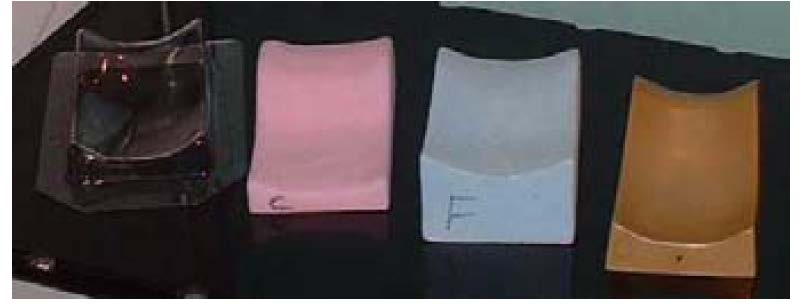
\includegraphics[width = 15cm]{images/ptpaid_01}
        \caption{caption.}
        %\label{fig:}
    \end{figure}

	\begin{figure}[!h]
	    \centering
        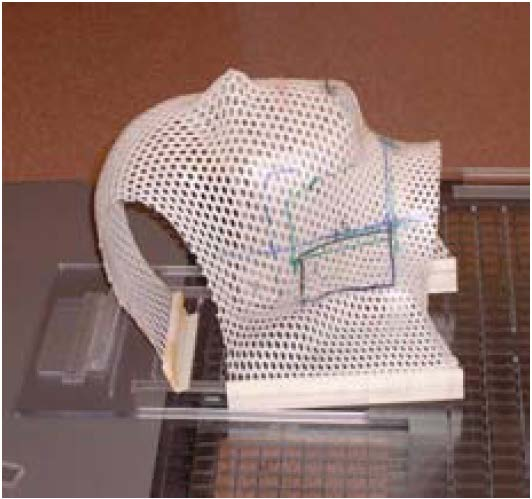
\includegraphics[width = 15cm]{images/ptpaid_02}
        \caption{caption.}
        %\label{fig:}
    \end{figure}

\chapter{თანამედროვე რადიაციული თერაპია (Modern Radiation Therapy)}
\section{სამგანზომილებიანი კონფორმალური რადიაციული თერაპია (Three-Dimensional Conformal Radiation Therapy)}
სამგანზომილებიანი კონფორმალური რადიოთერაპია (3-D CRT) ვგულისხმობთ მკურნალობას რომლებიც ეფუძნება 3-D ანატომიურ ინფორმაციას და იყენებს მკურნალობის ველებს, რომლებიც მაქსიმალურად შეესაბამება სამიზნე მოცულობას, რათა უზრუნველყოს ადეკვატური დოზა სიმსივნეზე და მინიმალური შესაძლო დოზა ნორმალურ ქსოვილზე. ონცეფცია დოზის კონფორმული განაწილება ასევე გაფართოვდა კლინიკურ მიზნებზე, როგორიცაა სიმსივნის კონტროლის ალბათობის მაქსიმიზაცია (TCP) და მინიმიზაცია ნორმალური ქსოვილის გართულების ალბათობა (NTCP). ამრიგად, 3-D CRT ტექნიკა მოიცავს ორივეს.

\section{დოზის მოცულობის ჰისტოგრამები (Dose Volume Histograms)}
დოზის განაწილების ჩვენება იზოდოზის მრუდების ან ზედაპირების სახით სასარგებლოა, რადგან ის აჩვენებს არა მხოლოდ ერთიანი დოზის, მაღალი დოზის ან დაბალი დოზის რეგიონებს, არამედ მათი ანატომიური მდებარეობა და ზომა. 3-D მკურნალობის დაგეგმვაში ეს ინფორმაცია აუცილებელია, მაგრამ უნდა გამყარდეს DVH-ებით სეგმენტირებული სტრუქტურებისთვის, მაგალითად, მიზნები და კრიტიკული სტრუქტურები. DVH არა მხოლოდ იძლევა რაოდენობრივ ინფორმაციას იმის შესახებ, თუ რა დოზა შეიწოვება რა მოცულობაში,  ასევე აჯამებს დოზის მთელ განაწილებას ერთ მრუდში თითოეული საინტერესო ანატომიური სტრუქტურისთვის.  ამრიგად, ეს არის შესანიშნავი ინსტრუმენტი მოცემული გეგმის შესაფასებლად ან კონკურენტ გეგმებთან შესადარებლად. DVH შეიძლება წარმოდგენილი იყოს ორი ფორმით: კუმულაციური ინტეგრალური DVH და დიფერენციალური DVH.  კუმულაციური DVH არის მოცულობის დიაგრამა მოცემული სტრუტურის, რომელიც იღებს გარკვეულ დოზას ან უფრო მაღალ დოზას. კუმულაციური DVH მრუდის ნებისმიერი წერტილი აჩვენებს მოცულობას, რომელიც იღებს მითითებულ ან უფრო მაღალ დოზას. დიფერენციალური DVH არის მოცულობის დიაგრამა, რომელიც იღებს დოზას განსაზღვრული დოზის ინტერვალის ფარგლებში (ან დოზის ურნა) დოზის ფუნქციის მიხედვით.

\section{ინტენსივობით მოდულირებული რადიაციული თერაპია (Intensity-Modulated Radiation Therapy)}
ტერმინი ინტენსივობით მოდულირებული რადიაციული თერაპია (IMRT) წარმოადგენს რადიაციას თერაპიის ტექნიკას, რომელშიც პაციენტზე ხდება არაერთგვაროვანი სხივებით ზემოქმედება სამკურნალო აპარატის ნებისმიერი პოზიციიდან, რათა ოპტიმირებული იყოს კომბინირებული დოზის  თანაბრად გადანაწილება. მკურნალობის გეგმის ოპტიმიზაციის კრიტერიუმები განისაზღვრება დამგეგმავის მიერ და ოპტიმალური ნაკადის პროფილები მოცემული მიმართულების სხივისთვის განისაზღვრება ინვერსიული დაგეგმარების საშუალებით. ამგვარად წარმოქმნილი ნაკადის ფაილები ელექტრონულად გადაეცემა ხაზოვან ამაჩქარებელს, რომელიც კომპიუტერით კონტროლდება, ანუ აღჭურვილია საჭირო პროგრამული უზრუნველყოფით და აპარატურით, რათა მიეწოდოს  ინტენსივობით მოდულირებით გამოთვლილი სხივები (IMBs).  IMRT-ის კლინიკური განხორციელება მოითხოვს მინიმუმ ორ სისტემას: (ა) სამკურნალო-დაგეგმვის კომპიუტერული სისტემას, რომელსაც შეუძლია გამოთვალოს არაერთგვაროვანი ნაკადის  გეგმები, სხვადასხვა მიმართულებით მიმართული მრავალჯერადი სხივების დოზის მაქსიმიზაციისთვის სამიზნე მოცულობაზე, კრიტიკულ ნორმალურ სტრუქტურებში დოზის მინიმიზაციისას და (ბ)  დაგეგმილი არაერთგვაროვანი ნაკადის მიწოდების სისტემა. თითოეული ეს სისტემა უნდა სათანადოდ დაისტესტოს ექსპლუატაციაში შესვლასა და რეალურ კლინიკურ გამოყენებამდე.

\section{სტერეოტაქსიური რადიოთერაპია და რადიოქირურგია (Stereotactic Radiotherapy and Radiosurgery)}
სტერეოტაქსიური რადიოქირურგია (SRS) არის ერთფრაქციული სხივური თერაპიის პროცედურა ინტრაკრანიალური დაზიანებების სამკურნალოდ. სტერეოტაქსიური აპარატების კომბინაციის გამოყენებით  ვიწრო მრავალჯერად სხივებთან, რომლებიც მიწოდებულია არათანაბარბრტყელი იზოცენტრული რკალებით. იგივე პროცედურას, როდესაც გამოიყენება მრავალჯერადი დოზის ფრაქციების მიწოდებისთვის, ეწოდება სტერეოტაქსიურ რადიოთერაპია (SRT). ორივე ტექნიკა მოიცავს სამგანზომილებიან გამოსახულებას დაზიანების ლოკალიზაციისთვის და მკურნალობის ჩატარების მიზნით. დოზის კონცენტრირებახდება სამიზნე მოცულობაზე და მაქსიმალურად იზოგება ნორმალური უჯრედები.

\section{გამოსახულებით სახელმძღვანელო რადიაციული თერაპია (Image-Guided Radiation Therapy)}
გამოსახულებით მართვადი რადიაციული თერაპია (IGRT)  შეიძლება განისაზღვროს, როგორც სხივური თერაპიის პროცედურა, რომელიც იყენებს გამოსახულებებს თერაპიის პროცესის სხვადასხვა ეტაპზე: პაციენტის მონაცემების მოპოვებისთვის, მკურნალობის დასაგეგმად, სიმულაციისთვისა და სამიზნე ლოკალიზაციის განსასაზღვრად მკურნალობამდე და მკურნალობის დროს. ტერმინ IGRT ს გამოვიყენებთ რადიოთერაპიის აღსანიშნად,რომელიც იყენებს გამოსახულებებს სამიზნის ლოკალიზაციისთვის მკურნალობამდე და მკურნალობის დროს.

\section{პროტონული ნაკადებით თერაპია}
პროტონებით სხივური თერაპიის დაგეგმვის ძირითადი პრინციპები არსებითად იგივეა როგორც ფოტონებისა და ელექტრონების შემთხვევაში. ეს მოიცავს 3D გამოსახულებიდან მონაცემების მიღებას, სამიზნე მოცულობისა და რიკს ორგანოების განსაზღვრას, ერთი ან მეტი სხივის დაყენებას, სხივების კუთხეებისა და ენერგიის განსაზღვრას, ველის დიზაინის შერჩევას, მკურნალობის პარამეტრების ოპტიმიზაციას, იზოდოზის განაწილების ჩვენებას, დოზის მოცულობის ჰისტოგრამებს (DVHs)  და ა.შ. ეს ყველაფერი დამოკიდებულია მოცემული პაციენტის მდგომარეობასა და სირთულეზე.
\medskip


\chapter{მითითებები}
ტესტ ტესტ ტესტ
\bibliography{bibliography.bib} 

\end{document}